\documentclass{article}
\usepackage{framed}
\usepackage{scrextend}
\usepackage{xcolor}
\definecolor{shadecolor}{RGB}{55, 0, 49}
\usepackage[spanish, english]{babel}
\usepackage[dvips,a3paper,centering,margin=2cm]{geometry}
\usepackage{multicol}
\usepackage[utf8]{inputenc}
\usepackage{color}
\usepackage{float}
\usepackage{colortbl}
\usepackage{tabulary}
\usepackage{multirow}
\usepackage{amsmath}
\definecolor{rb}{rgb}{0.025,0.5,0.9} 
\definecolor{na}{RGB}{255,255,255}
\definecolor{title}{RGB}{55, 0, 49}
\usepackage{graphicx}  
\pagestyle{empty}
\def\to{\rightarrow}
\begin{document}
\vspace*{-2cm}
\changefontsizes{14pt}
\hspace*{-1cm}
\begin{minipage}{0.2\linewidth}
\vspace{0.7cm}
\vspace*{-0.15cm}
\includegraphics[scale=0.12]{images/ifir.eps}
\end{minipage}
\vspace*{-0.4cm}
\begin{minipage}{0.6\linewidth}
\vspace*{0.7cm}
\begin{center}
\changefontsizes{15pt}
\hspace*{-0.1cm}
\textbf{\textcolor{title}{Desarrollo de la plataforma “TES para tu salud” que determina los Tiempos de Exposición Solar adecuados para el tratamiento de Psoriasis en la Ciudad de México}}
\end{center}
\vspace{-1cm}
\begin{center}
\begin{small}
    Gamaliel López-Padilla$^1$, Adriana Ipiña$^{2}$,Rubén Piacentini$^{2}$\\
    1. Facultad de Ciencias Físico-Matemáticas,UANL, México\\
    2. Instituto de Física Rosario,CONICET-UNR, Argentina\\
    email: giovannilopez9808@gmail.com, ipina@ifir-conicet.gov.ar
\end{small}
\end{center}
\end{minipage}
\begin{minipage}{0.2\linewidth}
\hspace*{0.2cm}
\includegraphics[scale=0.2]{images/fcfm.eps}
\end{minipage}
\vspace{0.25cm}
\begin{multicols}{2}
\changefontsizes{13pt}
\begin{center}
\begin{shaded}
\textbf{\textcolor{na}{Introducción}}
\end{shaded}
\end{center}
\begin{minipage}{0.4\linewidth}
\includegraphics[scale=0.35]{images/TES.png}
\vspace{-0.6cm}\\
\changefontsizes{0.5pt}
\textcolor{white}{Cortesía:Centro \\Dermatológico Pascua}
\begin{center}
\changefontsizes{10pt}
\vspace{0.6cm}
\textcolor{na}{Paciente afectado con Psoriasis}
\end{center}
\end{minipage}
\hspace{-0.cm}
\begin{minipage}{0.6\linewidth}
La Psoriasis es una enfermedad dermatológica crónica de apariencia de piel engrosada, que suele ser tratada con fototerapia ultravioleta (UV). Los pacientes son expuestos a fuentes artificiales UVA (320-400nm) siendo ésta la modalidad más utilizada en los Centros
\end{minipage}
 Médicos. Sin embargo, por diversos motivos los pacientes no tienen acceso a estos tratamientos o no pueden asistir con la asiduidad para recibirlo adecuadamente. Una recomendación alternativa es exponerse al sol. En este trabajo presentamos una  estimación de los tiempos de  exposición solar (TES)  en la ciudad de Monterrey para acumular las dosis UVA (Dosis$_{UVA}$) equivalentes a las suministradas en el tratamiento de Psoriasis.
\vspace{0.1cm}
\begin{center}
\begin{shaded}
\textbf{\textcolor{na}{Metodologia}}
\end{shaded}
\end{center}
\vspace{-0.3cm}
En este estudio utilizamos como referencia el máximo diario de la irradiancia solar visible e infrarroja-cercana (Vis+NIR*) medida por el Sistema de Monitoreo Ambiental (SIMA). Se filtran las mediciones bajo cielo despejado y con un código propio se fijan límites numéricos e ingresan al Modelo TUV 5.3.2 los parámetros atmosféricos así como las coordenadas de la ciudad de Monterrey$^{\left[1 \right]}$. Este se ejecuta hasta que la diferencia relativa porcentual entre medición y modelo es menor al 5\%. En este proceso se deriva del modelo la irradiancia solar espectral E$_{sol}$.
\begin{center}
    \begin{table}[H]
        \centering \normalsize
    \begin{tabulary}{1.0\linewidth}{ccccccc}
         \multirow{3}{*}{Phototype}&  & &&&&Skin color\\
         &	H$_{er}$ (SED)	& \multicolumn{4}{c}{Skin color} & of the\\ 
        &		&  &&& & Mexican population (\%)\\ \hline
        I 	&2.0	&\cellcolor[RGB]{251, 244, 227}\hspace*{0.05cm} 	&\cellcolor[RGB]{245, 240, 218}\hspace*{0.05cm}  &\cellcolor[RGB]{247, 238, 217}\hspace*{0.05cm} 	&\cellcolor[RGB]{248, 234, 209} \hspace*{0.05cm} &0.8	\\ \hline
        II 	&2.5	&\cellcolor[RGB]{248, 234, 208}	&\cellcolor[RGB]{247, 231, 206} &\cellcolor[RGB]{247, 223, 199}	&\cellcolor[RGB]{245, 222, 188}	& 3.9 \\ \hline
        III &3.0 	&\cellcolor[RGB]{245, 221, 188}	&\cellcolor[RGB]{238, 213, 170} &\cellcolor[RGB]{219,182,137}	&\cellcolor[RGB]{220,170,120} &24.0	\\ \hline
        IV 	&4.5	&\cellcolor[RGB]{219, 191, 129}	&\cellcolor[RGB]{208, 171, 107} &\cellcolor[RGB]{193, 150, 90}	&\cellcolor[RGB]{182, 135, 75}&59.2	\\ \hline
        V	&6.0	&\cellcolor[RGB]{172, 121, 68}	&\cellcolor[RGB]{135, 92, 50}  &\cellcolor[RGB]{113, 70, 38}	&\cellcolor[RGB]{77, 48, 28}&8.9	\\ \hline
        VI 	&10.0 	&\cellcolor[RGB]{68, 37, 20}	&\cellcolor[RGB]{43, 25, 8}  &\cellcolor[RGB]{32, 12, 7}	&\cellcolor[RGB]{10, 2, 5}	&2.5	\\ \hline
    \end{tabulary}
    \caption{{Adaptation of the Fitzpatrick classification for: skin phototypes,
            threshold erythemal dose in terms of Standard Erythemal Dose (SED), Skin
            colors and percentages (\%) of presence in the Mexican population
            {\label{290967}}%
    }}
    \end{table}
\end{center}
 \vspace{-0.5cm}
En cabina de fototerapia la Dosis$_{UVA}$ aplicada para Psoriasis es de 1J/cm$^2$ como fracción inicial$^{\left[2 \right]} $. Para obtenerla a partir de la irradiancia solar espectral se utiliza la siguiente ecuación:
\begin{equation*}
    Dosis_{UVA}=\int\limits_{t_1}^{t_2} \int\limits_{320nm}^{400nm} E_{sol}d\lambda dt= \int\limits_{t_1}^{t_2}I_{UVA}dt=1J/cm^2
\end{equation*}
donde t$_1$ y t$_2$ son la hora de inicio y hora de finalización de la exposición tal que la integral es igual a 1J/cm$^2$. Por lo tanto t$_2$-t$_1$ es el TES requerido$^{\left[3 \right]} $. La dosis UV eritémica (Dosis$_{erit}$) en un fototipo de piel caucásico es de 210 J/m$^2$. Para alcanzarla y determinar el TES correspondiente se incluye en la ecuación el espectro de sensibilidad eritémica $E_{erit}$ de la piel humana:
\begin{equation*}
    Dosis_{Erit}=\int\limits_{t_1}^{t_2} \int\limits_{290nm}^{400nm} \left( E_{erit}E_{sol}\right)d\lambda dt = \int\limits_{t_1}^{t_2}I_{erit}dt=210J/m^2
\end{equation*}
Las Dosis$_{erit}$ dependen del fototipo de piel por lo que pieles más morenas toleran TES más largos sin sufrir quemaduras.
\begin{center}
\begin{shaded}
\textbf{\textcolor{na}{Resultados}}
\end{shaded}
\end{center}
\vspace{-0.2cm}
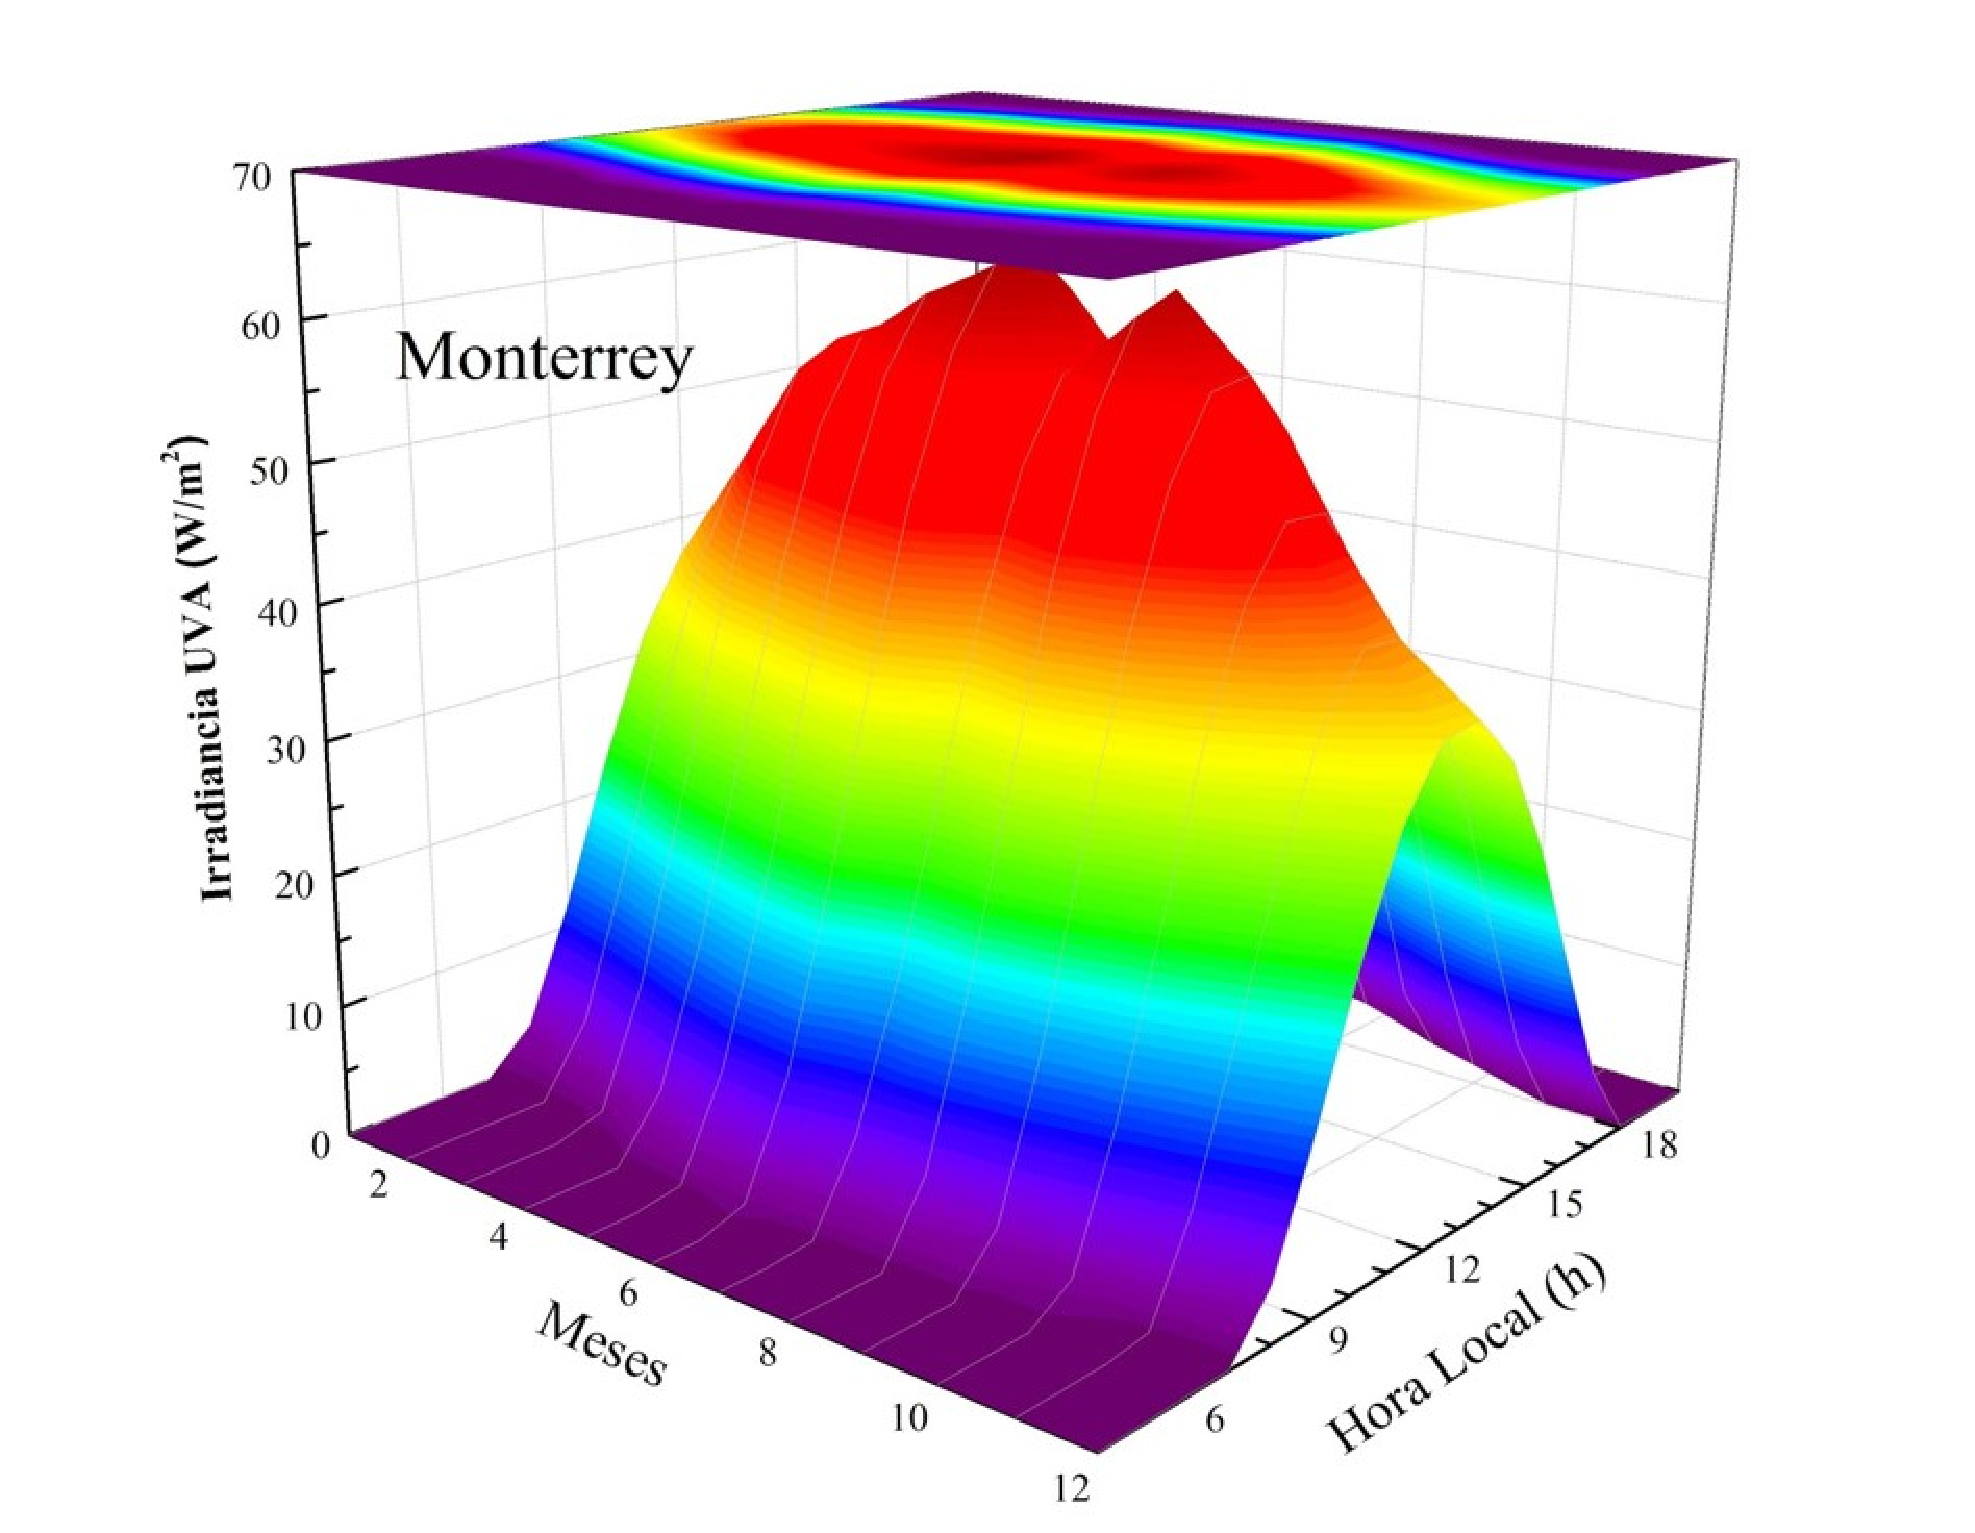
\includegraphics[scale=0.39]{images/pro.eps}\\
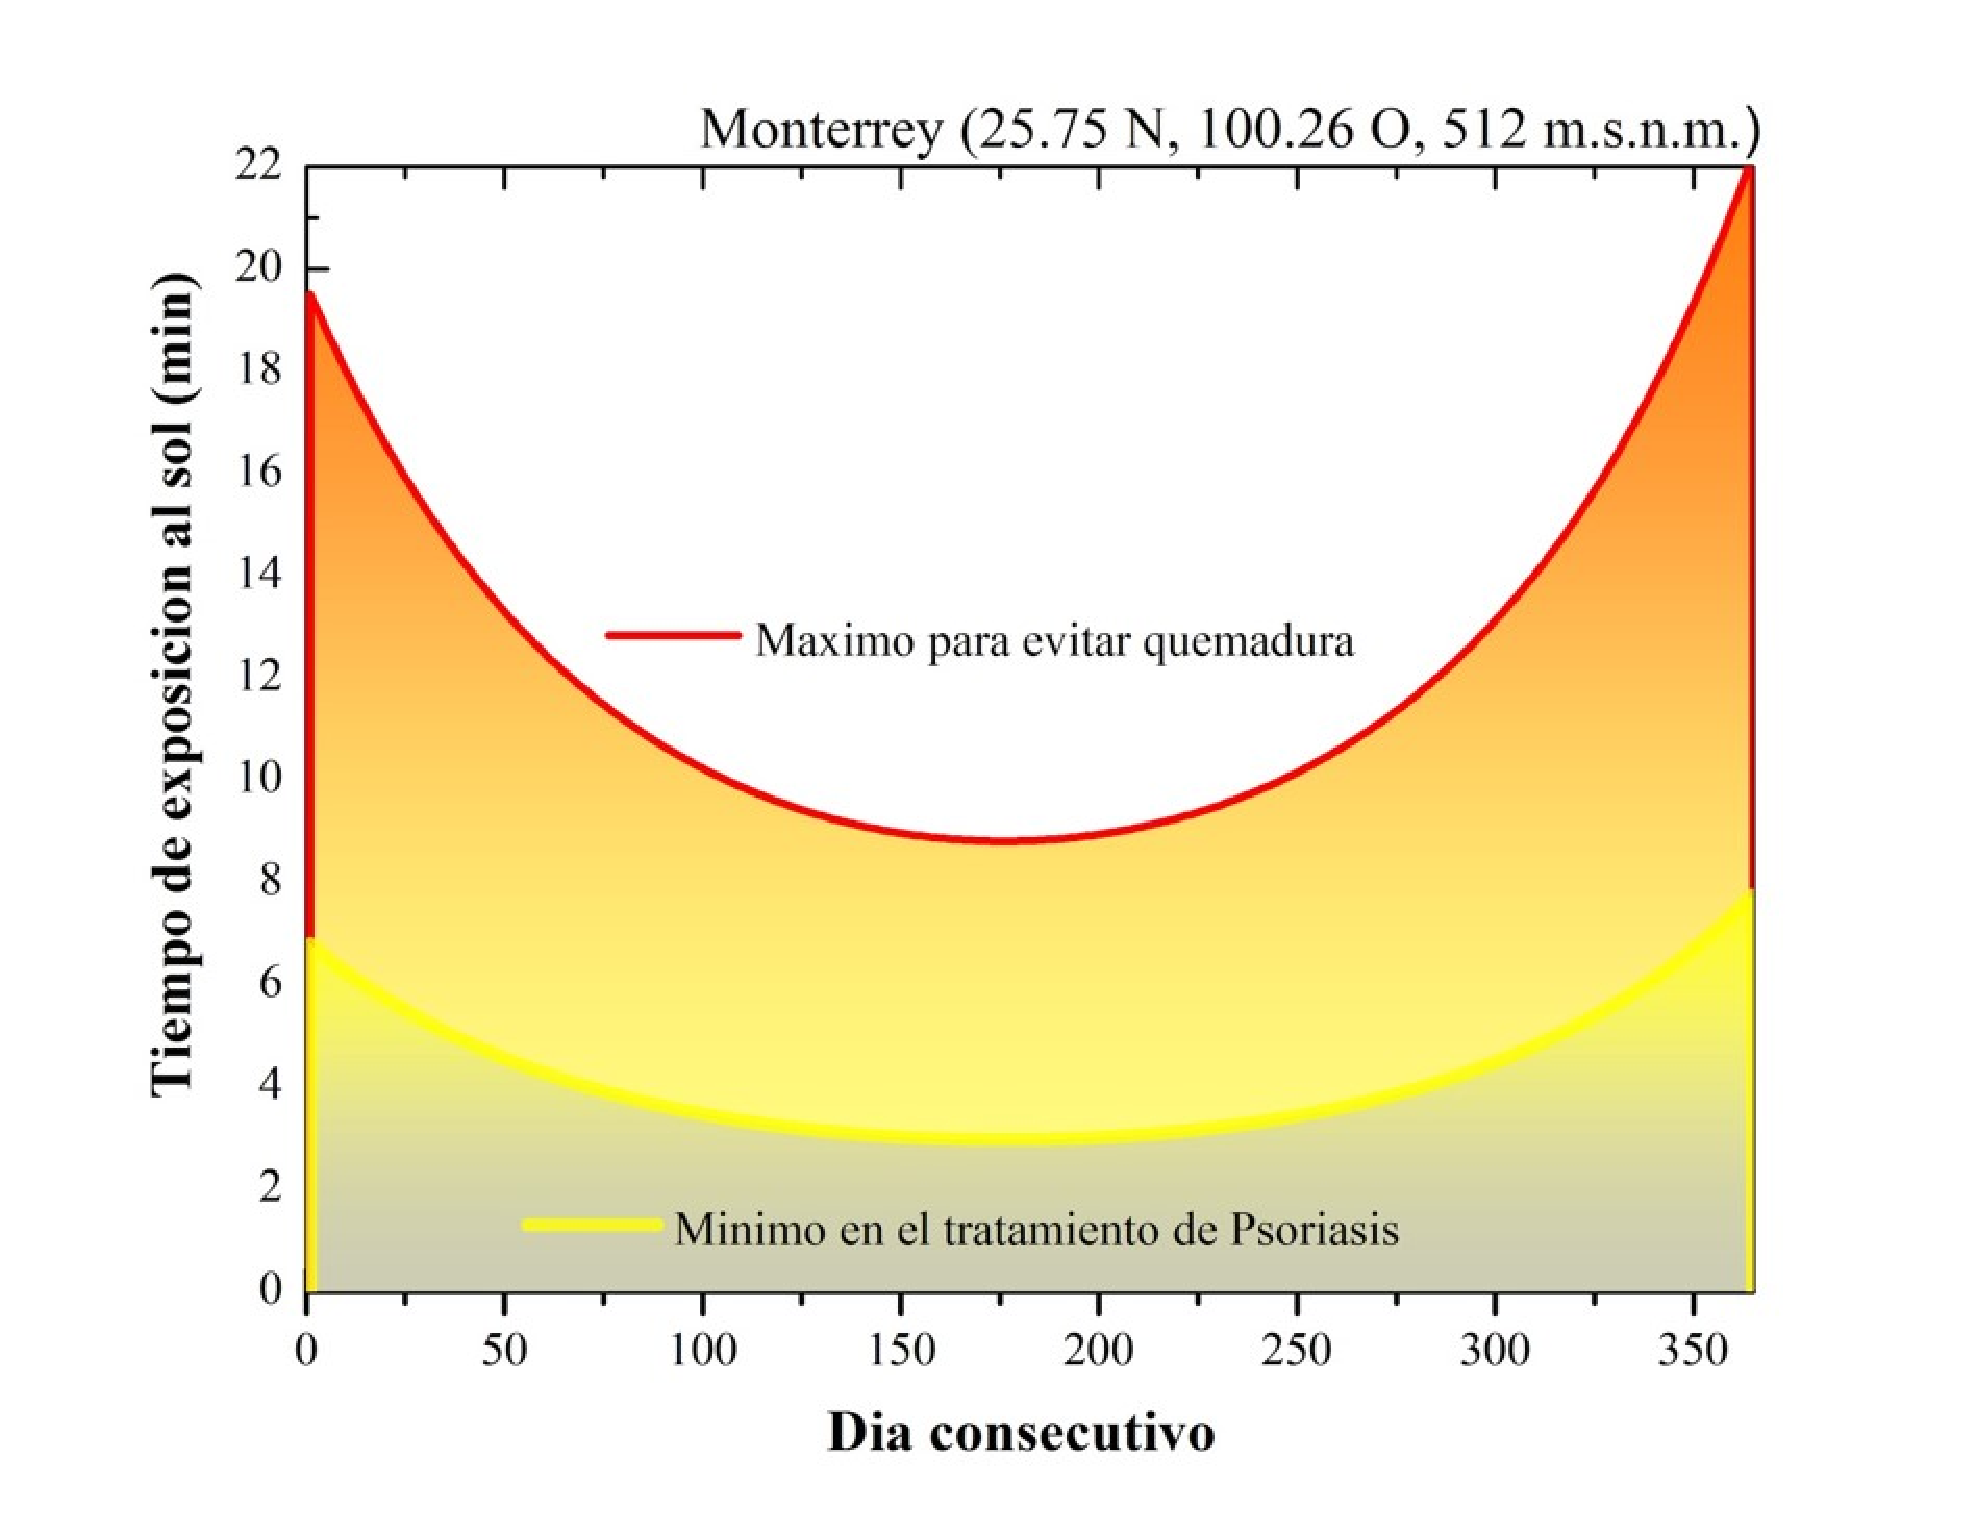
\includegraphics[scale=0.39]{images/ecua.eps}
\changefontsizes{10pt}
\textcolor{na}{I$_{UVA}$ calculada con Modelo TUV (sup). TES para acumular 1J/cm$^2$ de Dosis$_{UVA}$ y 210 J/m$^2$ de Dosis$_{erit}$ comenzando las 11:00 hs TL; funciones mínimas y máximas con coeficientes promedios anuales en el periodo 2015-2018 (inf).}
\changefontsizes{12pt}
\begin{center}
\begin{shaded}
\changefontsizes{12pt}
\textcolor{na}{Conclusiones}
\end{shaded}
\end{center}
\begin{minipage}{0.22\linewidth}
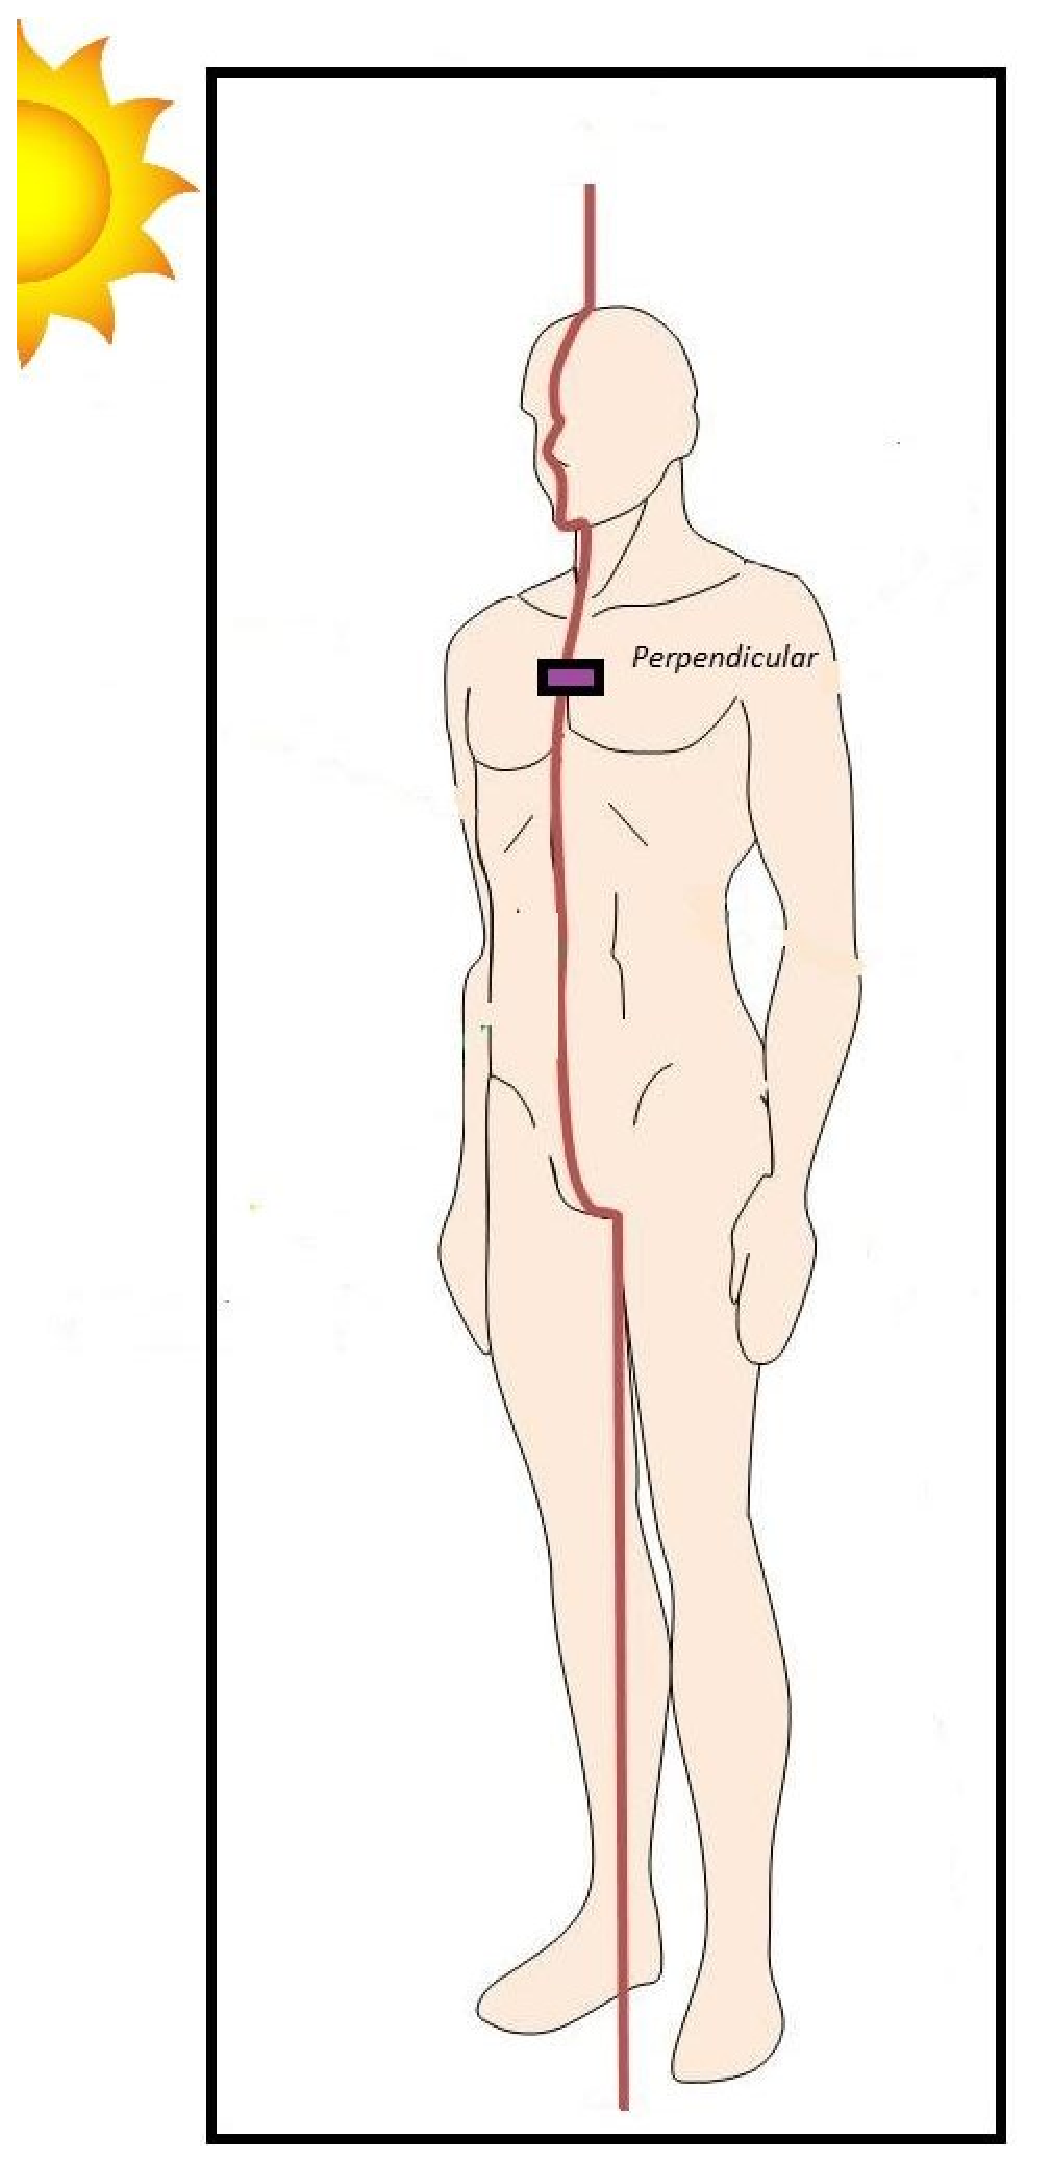
\includegraphics[scale=0.18]{images/cuerpo.eps}
\end{minipage}
\begin{minipage}{0.78\linewidth}
\begin{itemize}
    \item Los tiempos de exposición solar a lo largo del año, revelan que es factible alcanzar 1J/cm$^2$ equivalentes a las suministradas en fototerapia para Psoriasis.
    \item Por medio del modelo es posible determinar los tiempos de exposición límites para prevenir la quemadura solar.
    \item La helioterapia para Psoriasis pudiera aplicarse en cualquier lugar del área metropolitana de Monterrey en cielo claro, con supervisión dermatológica.
\end{itemize}
\end{minipage}
\begin{center}
    \begin{shaded}
    \textbf{\textcolor{na}{Referencias}}
    \end{shaded}
    \end{center}
    \changefontsizes{6pt}
    \begin{enumerate}
        \item[1]{Madronich} Madronich S. Madronich, Environ. UV Photob, 1-39, 1993
        \item[2]{Krzyscin} Krzyścin JW, Jaroslawski J, Rajewska-Wiech B, Sobolewski PS, Narbutt J, Lesiak A, Pawlaczyk M. JPPB 35–41, 2012.
        \item[3]{ipiña} Ipiña A, Castaño C, Dántola M L, Thomas A H. Solar Energy Journal, (109) 45–53, 2014.
    \end{enumerate}
\end{multicols}
\end{document}